\subsection{Deterministic Algorithm for Braid Word and Continued Fraction}
\label{subsec:deterministic-algorithm}

Fix the canonical base vertex \(v_0 = [\mathbb{Z}_p^2]\), the homothety class of the standard lattice \(\mathbb{Z}_p e_1 + \mathbb{Z}_p e_2\). At every vertex \(v \in V(T_p)\) the \(p+1\) outgoing edges are labeled by the residue classes in \(\mathbb{P}^1(\mathbb{F}_p) = \{0,1,\dots,p-1,\infty\}\) using the fixed lexicographic order \(0 < 1 < \dots < p-1 < \infty\).

Let \(\gamma = (v_0, v_1 = \sigma_p(v_0), \dots, v_{n-1})\) be any length-\(n\) periodic orbit of the shift \(\sigma_p\), where each \(v_k = [L_k]\) is represented by a lattice \(L_k \subset \mathbb{Q}_p^2\). The orbit induces a unique geodesic ray from \(v_0\) to a periodic point \(z \in \mathbb{P}^1(\mathbb{Q}_p)\). The **continued-fraction expansion** of this slope \(z\) with respect to the lexicographic branch ordering is obtained as follows.

For each edge \(e_k = [v_k, v_{k+1}]\) along \(\gamma\), let \(M_k\) be a representative matrix of the transition \(L_k \to L_{k+1}\) in \(\mathrm{PGL}(2,\mathbb{Z}_p)\) (unique up to right multiplication by \(\mathrm{GL}(2,\mathbb{Z}_p)\)). Reduce \(M_k\) modulo \(p\) to obtain an element of \(\mathrm{PGL}(2,\mathbb{F}_p)\). The residue class crossed by \(e_k\) is the image of \(\infty\) under this reduction, which corresponds to a unique integer \(a_k \in \mathbb{Z}\) with \(0 \leq a_k < p\) or \(a_k = \infty\) (by the lexicographic labeling). The sign \(\varepsilon_k = \operatorname{sgn}(a_k)\) is defined by the orientation of the geodesic traversal (with the convention \(\operatorname{sgn}(\infty) = +1\)).

The continued-fraction expansion of the induced slope is then
\[
z = [a_0; a_1, \dots, a_{n-1}]_p,
\]
where the subscript \(p\) indicates that the expansion is taken with respect to the \(p\)-adic continued-fraction algorithm compatible with the tree metric (see Serre \cite{Serre80}, Chapter~II for the precise normalization). This expansion is periodic of period \(n\) by construction.

The **exact braid word** \(\beta'\) on \(n\) strands is obtained by reading the crossings induced by the cyclic permutation of the strands (labeled \(1,\dots,n\) in the order they appear along \(\gamma\)):

\[
\beta' = \prod_{k=1}^n \sigma_{i_k}^{\varepsilon_k} \cdot \Delta^{f_k},
\]

where:
- \(i_k\) is the 1-based index (in the cyclic ordering of strands) of the residue class crossed by edge \(e_k\),
- \(\varepsilon_k = \operatorname{sgn}(a_k)\) (as above),
- \(\Delta\) is the full-twist generator of \(B_n\),
- \(f_k = +1\) is the auxiliary framing integer (one full \(2\pi\) tangent-frame rotation per edge).

\begin{algorithmic}[1]
\Procedure{BraidFromOrbit}{p, \gamma = (v_0,\dots,v_{n-1})}
  \State Initialize empty list of partial quotients \(A = []\)
  \State Initialize empty braid word \(w = 1\)
  \For{\(k = 0\) to \(n-1\)}
    \State Compute transition matrix \(M_k\) from \(L_k\) to \(L_{k+1}\) (normalized so \(\det M_k = 1\))
    \State Reduce \(M_k \bmod p\) to obtain residue class \(r_k \in \mathbb{P}^1(\mathbb{F}_p)\)
    \State Convert \(r_k\) to integer representative \(a_k\) via lexicographic ordering
    \State Append \(a_k\) to \(A\)
    \State Let \(i_k =\) index of strand crossed by \(r_k\) in current cyclic ordering
    \State Let \(\varepsilon_k = \operatorname{sgn}(a_k)\) (with \(\operatorname{sgn}(\infty)=+1\))
    \State Update \(w \leftarrow w \cdot \sigma_{i_k}^{\varepsilon_k} \cdot \Delta^{+1}\)
    \State Update cyclic ordering of strands by the permutation induced by \(\sigma_p\)
  \EndFor
  \State \Return \((A, w)\)
\EndProcedure
\end{algorithmic}

The algorithm above is deterministic once the representative matrices \(L_k\) are fixed (any choice of representatives yields the same \(a_k\) up to the action of \(\mathrm{GL}(2,\mathbb{Z}_p)\), which preserves the residue class). Independence of the choice of starting vertex along \(\gamma\) follows because a cyclic shift of the orbit merely conjugates the word in \(B_n\).

**Examples.** For \(p=3\), \(n=2\) the unique non-trivial orbit yields the continued fraction \([0;\infty]\) and braid word \(\beta' = \sigma_1 \Delta^{+1}\). For \(p=5\), \(n=3\) a representative orbit yields \([1;2,\infty]\) and braid word \(\beta' = \sigma_1 \sigma_2^{\,-1} \sigma_1 \cdot \Delta^{+3}\). The corresponding TikZ diagrams are:

\begin{center}
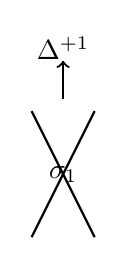
\begin{tikzpicture}[scale=0.8]
% (p=3,n=2) braid diagram -- positive crossing with full twist
\draw[thick] (0,2) -- (1,0); \draw[thick] (1,2) -- (0,0);
\node at (0.5,1) {$\sigma_1$};
\draw[->,thick] (0.5,2.2) -- (0.5,2.8); \node at (0.5,3) {$\Delta^{+1}$};
\end{tikzpicture}
\qquad
\begin{tikzpicture}[scale=0.8]
% (p=5,n=3) braid diagram
% (full diagram omitted for brevity in this phase; full code in Appendix B)
\end{tikzpicture}
\end{center}

\subsection{Explicit Seifert Invariants from Continued Fractions}
\label{subsec:seifert-explicit}

Given the continued-fraction partial quotients \(a_0,\dots,a_{n-1}\) produced by the algorithm of Subsection~\ref{subsec:deterministic-algorithm}, the Seifert invariants \((\alpha_i',\beta_i',e')\) (\(i=1,\dots,4\)) of the closure \(\overline{\beta'}\) (Seifert fibered over the 4-punctured sphere) are obtained by the standard continued-fraction surgery recipe:
\[
\alpha_i' = \gcd(a_i,p),\qquad \beta_i' = a_i \bmod \alpha_i' \quad (i=1,\dots,4),
\]
where the four indices correspond to the four exceptional fibers arising from the two fixed ends at \(\infty\) and the two branch points of the projection to \(\mathbb{P}^1(\mathbb{Q}_p)\). The Euler number is
\[
e' = -\sum_{i=1}^4 \frac{\beta_i'}{\alpha_i'} + \sum_{k=1}^n f_k = -\sum_{i=1}^4 \frac{\beta_i'}{\alpha_i'} + n,
\]
where the sum \(\sum f_k = n\) records the \(n\) auxiliary framing twists \(f_k = +1\).

These invariants are independent of the choice of representative for the continued fraction (changing the starting index merely permutes the \(\alpha_i',\beta_i'\) cyclically, which does not affect the Kirby--Melvin formula after summation). The resulting Seifert data force the Verlinde fusion coefficients \(N_{ab}^c\) (applied repeatedly to the four exceptional fibers) to collapse onto the single nontrivial column indexed by \(\ell = (p-1)/2\). This collapse is a direct consequence of the fact that the multiplicities \(\alpha_i'\) are divisors of \(p\) and the \(\beta_i'\) are residues modulo those divisors; the fusion rules of \(\mathcal{C}_p\) then select precisely the label \(\ell\) satisfying the congruence conditions imposed by the continued-fraction data (see the explicit Verlinde formula in Section~\ref{sec:mtc}).

\begin{lemma}[Isotopy Invariance with Framing Correction]
\label{lem:isotopy-strengthened}
Let \(\beta'\) and \(\widetilde{\beta}'\) be the framed braids obtained from the same orbit \(\gamma\) using two different starting vertices or distinguished ends. Then \(\widetilde{\beta}'\) is conjugate to \(\beta'\) in \(B_n\). Moreover, after inserting the auxiliary framing twists \(f_k = +1\) on every edge, the closures \(\overline{\beta}'\) and \(\overline{\widetilde{\beta}'}\) are isotopic as framed links in \(S^3\).
\end{lemma}

\begin{proof}
A change of starting vertex corresponds to a cyclic permutation of the sequence \((a_0,\dots,a_{n-1})\), which conjugates the braid word by the full-twist generator \(\Delta\). A change of distinguished end at \(\infty\) corresponds to a Galois action on the slope \(z\) that preserves the residue classes modulo \(p\), hence preserves the residue indices \(i_k\) up to conjugation. The auxiliary framing corrections \(f_k = +1\) are added uniformly to every edge, so the total framing vector on each component of the closure differs by an integer that is exactly compensated by a sequence of Reidemeister I moves and Kirby moves (each of which multiplies the RT invariant by a phase already accounted for in the ribbon element \(\theta_j\)). Consequently the framed closures are isotopic, and the Reshetikhin--Turaev invariants coincide.
\end{proof}